\section{Method}
\label{sec:method}
In this section, we describe the framework architecture and training procedure in detail.
Our intuition is to train a CNN that is capable of modeling the geometry consistency of a mostly rigid scene. To facilitate the learning of the network, we explicitly propose to model the constraint between depth and normal. The training samples of the framework consist of frame sequences captured by a monocular moving camera.
  
\subsection{Objective function}
To model a reasonable geometrical consistency, we propose the overall objective function as in Equation \ref{equ:1}.
\begin{equation}
\label{equ:1}
\begin{split}
L(D, I, Rt, \lambda) = L_{warp}(D, I, Rt) + L_{smooth}(D, N, I) \\
 +  L_{grad}(D, I, Rt) + \lambda(L_{dn}(D, N))
\end{split}
\end{equation}
This objective function is a Lagrange fuction aiming to minimize the loss term $L_{warp}(D, I, Rt) + L_{smooth}(D, N, I) \\
 +  L_{grad}(D, I, Rt)$ subject to the constraint of geometrical constraint between depth map and normal map $L_dn(D, N) = 0$. The loss term consists of three components: photometric warping loss $L_{warp}(D, I, Rt)$, smoothness loss $L_{smooth}(D, N, I)$, image gradient matching loss $L_{grad}(D, I, Rt)$.
 
\textbf{Photometric warping loss.} 
\label{chap:warping}
One main supervision of our framework comes from novel view synthesis: given an input view of a scene and camera motion, synthesize an image of the scene seen from a different view. We can synthesize an image of the target view given the image of source view, camera motion from target view to source view and depth map of target view, using 3D inverse warping. The process of warping is shown in Figure \ref{fig:3d_warping}.
\begin{figure}
\centering
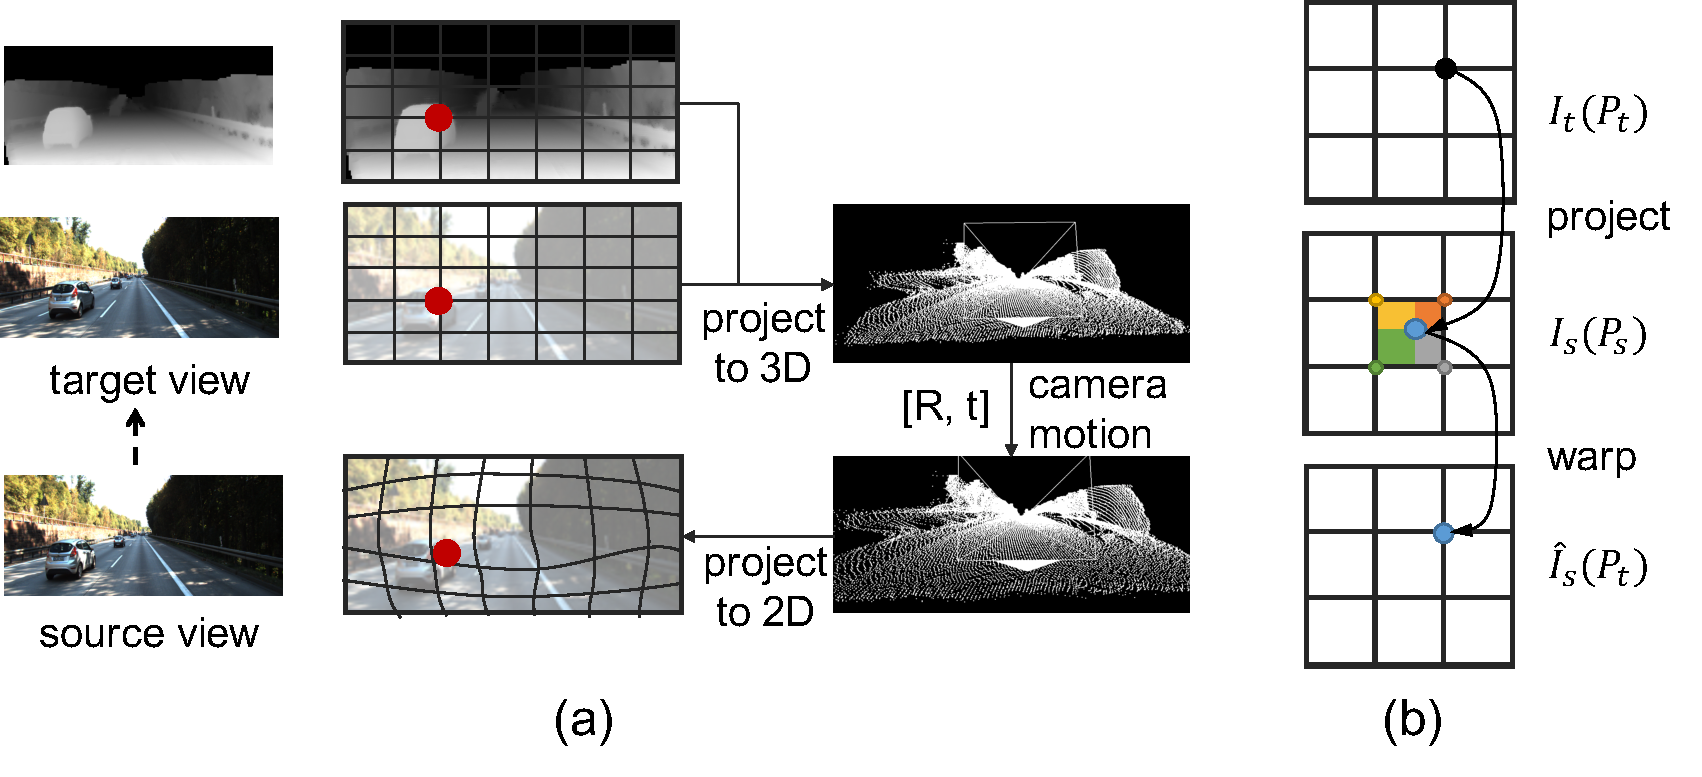
\includegraphics[width=0.5\textwidth]{figures/3d_warping.pdf}
\caption{Illustraion of (a) 3D inverse warping and (b) bilinear interpolation.}
\label{fig:3d_warping}
\end{figure}
Each pixel (point on the grid) of depth map is first mapped onto 3D space. The 3D point cloud is transformed based on camera motion and then mapped back to 2D plane. Each grid point in target view corresponds to one point in source view. Similar to \cite{jaderberg2015spatial}, the bilinear interpolation is implemented to calculate each pixel value of warped image as a weighted sum of four nearest neighboring pixels in source image, weighted by the square area between the projected point and neighboring point, as shown in Figure \ref{fig:3d_warping} (b).

The warping loss is a photometric difference between the target image and warped image. $$L_{warp}(D, I, Rt) = \sum_s\sum_p|I_t - \hat{I_s}|$$
In which, $s$ iterates the number of source image, $p$ iterates each pixel in the image, $I_t$ is the target image, $I_s$ is the source image, $\hat{I_s} = \tau(I_s, D_t, Rt)$ is the warped image, $\tau$ is the warping function as introduced above.

\textbf{Edge-aware smoothness loss.} One issue with using only view synthesis as supervision is that the back-propagation gradients are solely derived from the pixel value difference between one point in target image and weighted sum of its four neighboring points in source image. The warping loss will not be useful for learning where the point falls on low-texture regions. The predicted depth on these regions can be of any value as long as the warped region has the similar pixel value.  To overcome this issue, a prior knowledge of the scene geometry is incorporated for a smoothness loss:
\small
$$L_{smooth}(D) = \frac{1}{p} \sum_{p}(|\partial^2_xX_p|e^{(-\alpha||\partial_xI_p||)} + |\partial^2_yD_p|e^{(-\alpha||\partial_yI_p||)})$$
\normalsize

This smoothness term penalizes the norm of second-order gradients of depth in order to encourage smoothly changing depth values. As depth discontinuity often happens at image gradients, the smoothness loss is weighted by the a function of image gradients to prevent smoothed depth at image gradients. 

\textbf{Image gradient matching loss.}

To further facilitate the macthing of target image and warped image, and to encourage the depth map to be sharp, the photometric difference of gradient maps of target image and warped image is cacluated as gradient matching loss.
$$L_{grad}(D, I, Rt) = \sum_s(|\partial_xI_t - \partial_x\hat{I}_s| + |\partial_yI_t - \partial_y\hat{I}_s|)$$


\subsection{Geometry consistency}

As depth and surface normal are not independent under the same scene, 
thus we model the 3D geometry consistency by explicitly incorporating the relationship of depth and normal into the training procedure and use the relationship as a regularization in the objective function. The regularization term $L_{dn}(D,N) = 0$ is realized by two layers in our framework: depth2normal layer and normal2depth layer.

\textbf{Depth2normal layer.} 
\label{chap:d2n}
The normal direction of each point is computed based on the neighboring points after projecting to 3D space. The process of calculating normal direction of point $p$ is shown in Figure \ref{fig:d2n}. $\theta(p)$ is a set of neighboring (8) points of $p$. Take point $q \in \theta(p)$ for example. $R_{q}$ is a set of points that satisfy the requirement: when projecting to 3D space, for $\hat{q} \in \hat{\theta}(p)$ and for $\hat{r} \in \hat{R}_{q}$, $(\hat(q)-\hat(p) \cdot (\hat{r} - \hat(p)) \neq 0)$. Symbols with hat represent corresponding points in 3D space. Theoretically, the cross-product of any two non-collinear (in 3D space) vectors connecting $\hat{p}$ and $\hat{\theta}(p)$ is the normal direction $N(p)$. To reduce the possiblity that the two vectors being collinear in 3D space, we require the vectors to be perpendicular when projected in 2D plane. The normal directions are averaged when iterating $q \in \theta(p)$, and then $l_2$ normalized to make it a unit vector. The normal direction is calculated as:
$$N(p) = l_2(\sum_{\theta(p)}\sum_{R_q}((\hat{q} - \hat{p}) \times (\hat{r} - \hat{p}))) \quad q \in \theta(p), r \in R_q$$
for each $q\in\theta(p)$, $R_q$ satisfies $(q-p)\cdot(r-p) = 0, \quad r \in R_q$.

\begin{figure}
\centering
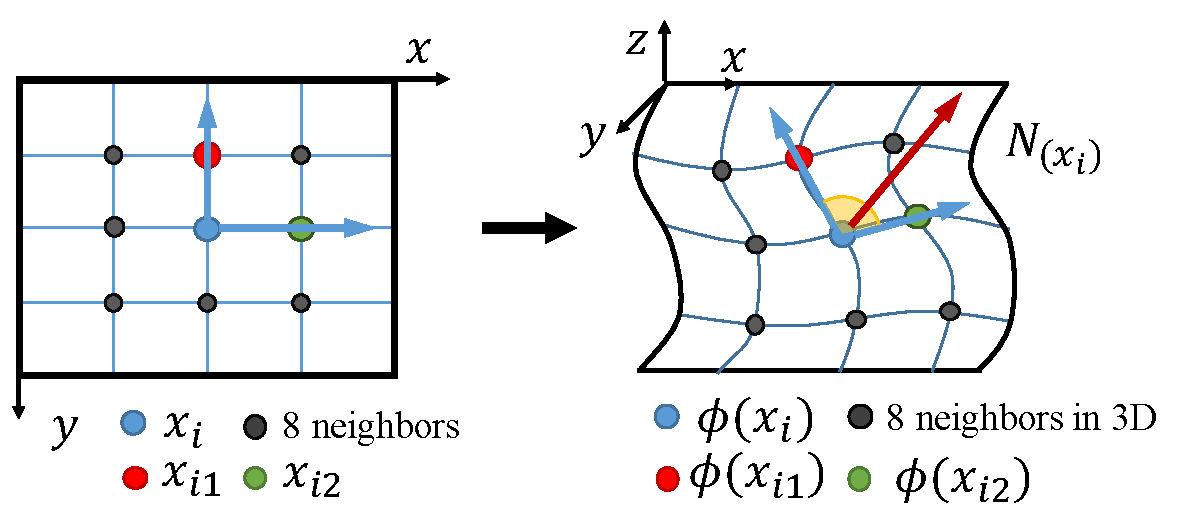
\includegraphics[width=0.5\textwidth]{figures/d2n.pdf}
\caption{Depth2normal layer. $p, q, \theta(p), q_{\theta(p)}$ are 2D points, and $\hat{p}, \hat{q}, \hat{\theta}(p), \hat{q}_{\theta(p)}$ are corresponding points projected to 3D space.}
\label{fig:d2n}
\end{figure}

\textbf{Normal2depth layer.} Normal2depth layer takes depth map and normal map as input and outputs a ``shifted" depth map. Take Figure \ref{fig:d2n} for example, the depth values of points $\theta(p)$ can be calcuated with the depth and normal direction of point $p$ known. From the calculation of normal direction, $(\hat{p} - \hat{q}) \cdot N(p) = 0$. When projecting points from 2D plane to 3D space, $\hat{p} = K^{-1}p$. $\hat{p} = (\hat{x}_p),\hat{y}_p,\hat{z}_p$, $p = (x_p, y_p, z_p)$ is a homogeneous 2D point and $z_p$ is the depth value of point $p$. $K^{-1}$ is the inverse of intrinsic matrix, which is determined by the camera. In linear the equation between depth and normal direction, $(K^{-1}(x_p, y_p, z_p) - K^{-1}(x_q, y_q, z_q))\cdot N(p) = 0, q\in\theta(p)$, the only unknown $z_q$, \ie  depth value of point $q$, has a unique solution. 

As there are multiple points in the set $\theta(p)$, multiple depth maps can be recovered corresponding to each point $q \in \theta(p)$. In our pratice, the $\theta(p)$ includes 8 nearest points around point $p$. The 8 depth maps are weighted averaged to produce a reasonable depth output. As depth and normal discontinuity often happens where image gradients are large, similar to using image gradient in smoothness loss term, the image gradients are also calculated as weights to determine how much of each depth map contribute to final output. The output depth map is calculated as:
$$z_p = \sum_{\theta(p)}z_q\frac{e^{(-\alpha|\partial_{\overrightarrow{p-q}}I_p|)}}{\sum_{\theta(p)}e^{(-\alpha|\partial_{\overrightarrow{p-q}}I_p|)}}, q\in\theta(p)$$
In which, $\partial_{|\overrightarrow{p-q}}I_p|$ is the image gradient value along the $\overrightarrow{p-q}$ direction.

\textbf{Network architecture.} Similar to \cite{zhou2017unsupervised} and \cite{godard2016unsupervised}, we adopt the DispNet \cite{mayer2016large} architecture with skip connections as in \cite{zhou2017unsupervised}. All \textit{conv} layers are followed by a ReLU activation except for the top prediction layer. 